\includeonly{
  slide-title,
  slide-introduction,
  slide-amr,
  slide-parallel,
  slide-conclusions
}

%%%%%%%%%%%%%%%%%%%%%%%%%%%%%%%%%%%%%%%%%%%%%%%%%%%%%%%%%%%%%%%%%%%%%%%%%%%%
%    This LaTeX source was automatically generated by outlinebeamer.pl     %
%                                                                          %
%   Remember that most changes should be made to the outline source file   %
% changes to this file will be overwritten when the file gets regenerated  %
%                                                                          %
%                  outlinebeamer - Outline Beamer Class Presentation Maker %
%                                    http://outlinebeamer.sourceforge.net/ %
%%%%%%%%%%%%%%%%%%%%%%%%%%%%%%%%%%%%%%%%%%%%%%%%%%%%%%%%%%%%%%%%%%%%%%%%%%%%
%\documentclass{beamer}

% --------------------------------------------------
%
% INTRODUCTION: ENZO-P / CELLO
%    
% --------------------------------------------------
%
% PARAMETERS
%
%   * Problem definition
%     - Enzo:  problem definition in code ("problem_type") and parameter file
%     - Enzo-P problem definition in parameter file
%     - requires much more flexible parameter files
%       - hierarchical organization
%       - more types 
%       - more difficult to implement
%       - flex for lexical analysis, bison for parsing
%         - generates C-code, which is thoroughly tested
%   * Parameter files
%     * parameters organized into "groups" and "subgroups"
%     * parameter types much more flexible than Enzo
%     * Enzo-P developers can trivially add new parameters:
%        parameters->set_current_group("Physics");
%        bool physics_on = parameters->("enable_physics",true);
%   * Parameter file example: Implosion problem
%   * Parameter file example: Collapse test
%   * Parameter file data types
%
%     - integer
%     - scalar
%     - logical
%     - string
%     - list
%     - scalar expression, 
%     - logical expression
%   parameters: hierarchical
%   parameters: expressive data types
%   parameters: easy to add new parameters: just use [API example]
%   parameters: compare parameter files with Enzo [implosion]
%   - initial conditions
%     - scalar expression "if-else" list
%     - input file
%     - user "initial" method
%
% --------------------------------------------------
%
% CODE DESIGN
%
%   Components
%   Component summary
%   - organized into "component" subdirectories
%   - e.g. Mesh, Field, Particles, Parameters
%   - Enzo-P code goes in User component
%   - data structures only manipulated directly from own class
%     - standard iterator functions for traversing complicated data structures
%       - [ hypre-solve code ]
%   
%
%
% --------------------------------------------------
% 
% AMR COMPONENT
%
%  * AMR variants
%    - "Structured" AMR
%      - e.g.~Enzo, Chombo, SAMRAI
%    - "Octree-based" AMR
%      - e.g.~Flash, ...
%  * Scalable AMR is an unsolved problem
%      - SAMR has scalablity issues
%        - gridding algorithm has scaling issues
%        - parent-child communication 
%        - scheduling/balancing variable-sized tasks
%      - Octree-AMR has scalability issues
%         - fixed-size patches inefficient for "shallow" AMR
%         - refining a single point involves entire root-level patch
%         - octree refinement inefficient for "deep" AMR
%     - Enzo-P: modified "octree-based" AMR
%       - similar to e.g. Flash, but with several (currently proprietary) enhancements
%       - improved scalability:
%         - fully distributed metadata
%         - only data transfer is between adjacent grid patches
%           - no parent-child
%       - improved performance
%         - patches subdivided into "blocks" (cache-friendly)
%         - unigrid is single AMR patch of blocks
%         - a timestep on a block is a single parallel task
%       - enhancements for "wide" problems (large regions at same level)
%         - Basic octree with fixed-sized blocks refines too much
%           - Flash patch count proportional to refinement area * $8^{level}$
%           - Enzo-P patch count proportional to refinement-change area $8^{level}$
%           - [figure]
%           - Enzo patch count good, but smaller patches at finer levels
%       - enhancements for "deep" problems (many refinement levels)
%         - octree refinment not "targeted": single point involves entire domain
%         - we will allow refinement by 4 and possibly 8
%            - still maintain smooth level jumps by 2 everywhere
%         - will address integer index range issues
%         - will address floating point positional precision issues
%       - reduced operations for physics modules compared to SAMR
%         - cubical typically small blocks
%         - limited inter-block configurations [ figure ]
%   * Cello AMR philosophy
%     - "AMR hierarchy" defines changes in resolution
%     - "AMR patch" defines areas of uniform resolution
%     - hierarchy size should be proportional to "amount" of resolution change
%       - not true of standard octree AMR (Flash) due to fixed-size patches
%       - not strictly true of Enzo AMR due to unigrid level (hierarchy = O(P^2)[?])
%     - Cello adds a new "level" to AMR
%       - "AMR block" defines task size
%       - typically small, e.g. $4^3$ to $8^3$
%       - a patch is composed of one or more blocks
%       - unigrid problem is single patch
%       - decouples "uniform resolution" requirements from "parallel task size"
%     - AMR 
%   AMR:        totally new AMR approach: generalization of octrees--rationale
%   AMR:        additional level of refinement: patches + blocks
%   AMR:        new [currently proprietary] enhancement for "large, shallow" AMR
%   AMR:        new [currently proprietary] enhancement for "deep, targeted" AMR
%   AMR:        no level jumps, symmetric refinement for symmetric problems
%   AMR:        ghost zones optionally allocated only when needed
%   AMR:        octree node memory footprint is light: 3 pointers (24 bytes) per patch
%   AMR:        optional fully distributed AMR hierarchy
%   scalability: Only adjacent block communication--no parent/child communication
%   scalability: Optional fully-distributed hierarchy (local patch + neighboring "ghost" patches)
%   performance: block sizes can be fixed (or at least quantized, e.g. $4^3$ $8^3$ or $16^3$), reducing memory fragmentation, improving cache utilization
%   performance: AMR enhancements will greatly reduce metadata
%   problem support: Deep: integer range and floating point precision
%   problem support: Deep: "level windows" to reduce memory usage
%   problem support: AMR enhancements for targeted refinement by 4 or 8 ["backfill" to maintain level jumps at most 2]
%
% --------------------------------------------------
%
% FIELD COMPONENT
%
%   Field:      data layout controlable from parameter file: ordering, padding, alignment, [interleaving]
%   Field:      default precision specified in parameter file, can be overridden for individual fields (may require promoting before passing to computational kernals)
%   Field:      ghost zone depth  specified in parameter file, can be overridden for individual fields
%   Field:      minimum/maximum values for fields optionally specified in input file, including action (warning, error, reduce time step, alternate method)
%   
%   Field:      fields explicitly specified in parameter file
%   Field:      field groups specified in parameter file (e.g. "color", etc.)
%   Issue: units?
%
% --------------------------------------------------
%
% USER COMPONENT
%
%  - Cello is designed to be a general-purpose "extreme AMR" framework
%  - "User" component is designed to hold application-specific
%   Enzo-P:     All Enzo physics code in User component
%   Enzo-P:     Includes methods (block advance, face update), timestep determination, control (ala EvolveLevel)
%      UserMethod:     basic method, initialization, analysis functions
%      UserCorrect:  "flux-correction" type operations at level interface boundaries
%      UserBoundary:  user-defined boundary conditions
%      UserTimestep:  user-defined timestep control (ala EvolveLevel)
%      UserRefinement user-defined refinement criteria
%      UserBalance    user-defined load balancing
%      UserSchedule   user-defined task scheduling
%      User????       other functions required?

% --------------------------------------------------
%
% MEMORY COMPONENT
%
%  - optionally fill memory with NaN after allocate
%    - help catch access of uninitialized data
%  - optionally fill memory with Nan before deallocate
%    - help catch access of unallocated data
%  - optionally track current / high memory per process
%  - optionally warn when memory threshold reached
%  - fixed (quantized) field (particle) block sizes
%    - should help reduce memory fragmentation
%  - can wrap other memory management libraries
%
% --------------------------------------------------
%
% PORTAL COMPONENT
%
%  * interact with external utilities
%    - yt, jacques, etc.
%  - inter-application communication using Parameters-like API
%    - probably XML
%    - read commands to retrieve data
%    - write commands to control simulation
%  * Example uses
%    - control
%      - modify simulation parameters as it progresses
%      - maintain log so results can be reproduced
%    - locate
%      - dynamically look for and track features
%    - analyse
%    - visualize
%      - e.g. contral a dynamic camera position, direction, frequency sensitivity, etc.
%    - performance
%      - find performance problems
%      - dynamically modify parameters to correct
%
%  * user-driven dynamic analysis
%    - more efficient than a posteriori analysis
%      - no large disk dumps
%    - more flexible than inline analysis
%      - discover and analyse features at run time
%      - all data available
%    - can dynamically change what data to store for later analysis
%      - useful if analysis would otherwise slow the computation
%
% --------------------------------------------------
%
% SOFTWARE ENGINEERING AND QUALITY CONTROL
%
% - prototyping
%   - proof-of-concept
%   - iron out design issues
%   - proven technique
% - testing
%   - unit testing integrated with code build (scons not make)
%   - integration tests how classes/components interact
%   - system tests entire application
%   - regression testing
%   - test for previously-found bugs to prevent their reappearance
% - code reviewing
%   - goal: every line of code is proof-read
%   - proven effective
% - combining techniques more effective than individual
%   - computers tend to find different kinds of bugs than people

% --------------------------------------------------
%
% OUTPUT
%
%   Output:     Currently HDF5 and IFrit files supported
%   Output:     Different output 'types', restart, data, visualization, analysis, etc.
%
% --------------------------------------------------
%
% ERROR
%
%   Fault-tolerant design
% --------------------------------------------------
%
% PARALLELISM
%
%   parallel:   hierarchical: distributed-memory, shared-memory [GPU level]
%   parallel:   any level can be parallelized with different parallel technology (MPI,UPC,etc.)
%   parallel:   load balancing approach specified in parameter file, may be user-defined.  Initially space-filling curve, ultimately hierarchical diffusion
%   parallel:   fully distributed data structures (no / fixed global metadata)
%   Schedule, Balance, Task [ uml ]
%  
%     - dynamic parallel task creation / scheduling / migration
%       [ enzo is more static ]
%       [ remove unnecessary synchronization, e.g. between levels ]
%
% --------------------------------------------------
%
% FEEDBACK
%
%   % Limitations
%   * Enzo-P limitations
%     - cubical domains
%       - may be able to bypass
%         - use subset of domain
%         - set boundary conditions at internal positions
%         - need to refine along physical boundary for accuracy
%         - mask-out unused patches / blocks
%
% --------------------------------------------------
%
% CURRENT STATUS AND ROADMAP
%
% Initial Unigrid Release "Soon"
%
%   * Pre-release
%     - unigrid only
%     - PPM hydro only
%     - MPI only
%     - Why use it?
%       - flexible parameter files
%       - hopefully faster and more scalable
%         - adjustable field ordering, alignment, padding
%         - multiple data blocks per process (more cache friendly)
%         - treats unigrid as unigrid, not as AMR
%       - I need feedback
%
% Roadmap
%
%   + gravity (FFT(Harkness) or multigrid)
%   + PPML (with Kritsuk and Ustyugov
%   + AMR (after development and paper)
%
%   roadmap:    available now: Fields, Parameters, serial unigrid PPM
%   roadmap:    available imminently: parallel unigrid MPI-[12] PPM, PPML, gravity (FFT or MG)
%   roadmap:    available next: basic AMR (octree), local physics 
%   roadmap:    longer-term: particles, cosmology, enhanced AMR
%   roadmap:    papers: AMR enhancements
%   roadmap:    
%   development: extensive unit tests built into build
%   development: scons instead of make: advantages [disadvanteges]
%   development: currently subversion is sufficient--no branching
%   development: "physics" part separate from parallelism and data structures
%   problem support: Deep: integer range and floating point precision
%   problem support: Deep: "level windows" to reduce memory usage
%   problem support: AMR enhancements for targeted refinement by 4 or 8 ["backfill" to maintain level jumps at most 2]
%   feedback:  parameters
%   feedback:  functionality
%   feedback:  
%
% SLIDES
%
% * Enzo-P / Cello summary
%   
% * Why Enzo-P?
%    
% --------------------------------------------------
%
% CONCLUSIONS
%
%
% --------------------------------------------------

\documentclass{beamer}

\usetheme{Copenhagen}
\usecolortheme{default}

\newcommand{\Code}[1]{\textsf{#1}}
\newcommand{\cello}{\textsf{Cello}}
\newcommand{\enzo}{\textsf{Enzo}}
\newcommand{\enzop}{\textsf{Enzo-P}}
\newcommand{\code}[1]{\texttt{#1}}
\newcommand{\us}[1]{\color{blue}{#1}}
\newcommand{\them}[1]{\color{red}{#1}}
\newcommand{\newus}[1]{\color{magenta}{#1}}
\newcommand{\good}{\textcolor{green}{\smiley}}
\newcommand{\bad}{\textcolor{red}{\frownie}}
\newcommand{\colorcode}[1]{\textcolor{blue}{\code{#1}}}
\newcommand{\itemnum}[1]{\item<#1>}

%========================================================================
% UNCOMMENT TO PRINT
%========================================================================

 \newcommand{\enhance}[1]{}
 \newcommand{\enhancebf}[2]{\textbf{#2}}
 \newcommand{\enhanceus}[1]{\color{blue}}
 \newcommand{\enhancenewus}[1]{\color{magenta}}
 \newcommand{\enhancethem}[1]{\color{red}}
\newcommand{\ENHANCE}[1]{
 \temporal<#1>{\color{lightgray}}{\color{black}}{\color{gray}}}

%========================================================================
% UNCOMMENT FOR TALK:
%========================================================================

% \newcommand{\enhance}[1]{\temporal<#1>{\color{lightgray}}{\color{black}}{\color{black}}}
%  \newcommand{\enhancebf}[2]{\enhance{#1}\textbf{#2}}
%  \newcommand{\enhanceus}[1]{\temporal<#1>{\color{lightgray}}{\color{blue}}{\color{blue}}}
%  \newcommand{\enhancenewus}[1]{\temporal<#1>{\color{lightgray}}{\color{magenta}}{\color{magenta}}}
%  \newcommand{\enhancethem}[1]{\temporal<#1>{\color{lightgray}}{\color{red}}{\color{red}}}
% \newcommand{\ENHANCE}[1]{
%  \temporal<#1>{\color{lightgray}}{\color{black}}{\color{black}}}
%========================================================================


% \def\enhanceus<#1>{%
%  \temporal<#1>{\color{lightgray}}{\color{blue}}{\color{blue}}}
% \def\enhancenewus<#1>{%
%  \temporal<#1>{\color{lightgray}}{\color{magenta}}{\color{magenta}}}
% \def\enhancethem<#1>{%
%  \temporal<#1>{\color{lightgray}}{\color{red}}{\color{red}}}


\author{James Bordner}
\date{June 28, 2010}
%======================================================================
\begin{document}

\begin{frame}
\titlepage
\end{frame}


%========================================================================
% SECTION PAGES [ COMMENT FOR PRINT ]
%========================================================================
%\frame{\footnotesize
%\tableofcontents
%}
% \AtBeginSection[]
%{
%------------------------------------------------------------------------
%  \begin{frame}<beamer>
%\footnotesize
%   \tableofcontents[currentsection]
%  \end{frame}
%}
%========================================================================

\section{Introduction}
  \begin{frame}[fragile] 
%--------------------------------------------------
\frametitle{Project Motivation}
%--------------------------------------------------
\begin{itemize}
  \item Enzo development began around 1994
  \item Largest machine in 6/1994 had 3680 processors
  \item \textcolor{white}{Largest machine in}  6/2010 has 294912 cores
  \item \textcolor{white}{Largest machine in}  6/2026 will have 20000000 quorlets
  \item What will \enzo\ look like in 2026?
    \begin{itemize}
      \item let's not go there...
    \end{itemize}
  \item \enzo-P is being designed to be the next generation of \enzo
    \begin{itemize}
      \item Long-range goals to complement \enzo's shorter-range goals
      \item Maintain \enzo's beloved physics capabilities
       \item Redesign distributed AMR infrastructure
       \item Implemented on a general ``extreme-AMR'' framework: \cello
    \end{itemize}
\end{itemize}
\end{frame}

\begin{frame}[fragile] 
%--------------------------------------------------
\frametitle{Project Goals}
%--------------------------------------------------
\enzop\ / \cello\ design goals:
\begin{itemize}
  \item Highly scalable
    \begin{itemize}
      \item\enhance{2} parallel scalability (nodes, processors, cores)
      \item\enhance{3} data structure scalability (zones, grids, levels)
    \end{itemize}
  \item\enhance{4} Easy to use
    \begin{itemize}
      \item\enhance{5} simplified build system
      \item\enhance{6} enhanced parameter file grammar and syntax
    \end{itemize}
  \item\enhance{4} Easy to modify and enhance
    \begin{itemize}
      \item\enhance{5} object-oriented design
      \item\enhance{6} losely-coupled components
    \end{itemize}
\end{itemize}
\end{frame}

%------------------------------------------------------------------------
\begin{frame}[fragile] \frametitle{Extreme Scaling Issues}
   \begin{itemize}
      \item \enhance{1}Parallel task size control
      \begin{itemize}
          \item \enhance{1}Large enough for efficiency
          \item \enhance{1}Small enough for sufficient parallelism
      \end{itemize}
      \item \enhance{1}Global synchronization
      \begin{itemize}
          \item \enhance{1}Integration is level-by-level
          \item \enhance{1}Timestep determination
      \end{itemize}
      \item \enhance{2}SAMR gridding algorithm
      \item \enhance{3}Load balancing (nodes, processors, cores)
      \item \enhance{5}Software resiliency / fault tolerance
      \item \enhance{6}Checkpoint / restart
      \item \enhance{7}Numerical issues (index ranges, position precisions)
   \end{itemize}
\end{frame}
%   * Goals
%     - scalable to O(10^6) and beyond
%       [ redesign data structures to be highly-scalable from the start ]
%     - software resiliency
%       [ hardware components *will* fail ]
%     - dynamic parallel task creation / scheduling / migration
%     - improved user experience [ compilation, parameter files ]
%     - improved developer experience
%       - design is component-based: one directory per component
%       - loosely-coupled ``physics'' and ``computer science'' components
%         - Enzo-P: physics part
%         - Cello: computer science part
%     - quality control
%       - improved software development process
%       - requirements, design, implement, test
%     - enhanced capabilities
%       - AMR enhancements for both "deep" and "wide" problems
%       - built-in interface to interact with external applications
%         - visualization, analysis
%
%   * Capabilities
%   * Scalability and performance
%     - parallel scaling
%       - dynamic task scheduling
%         - allow patch-local timestepping: no global synchronization 
%     - data structure scaling
%       - positional floating point precision problems addressed
%         - local (patch) coordinate systems only
%       - integer index ranges addressed
%         - relative (neighbor) indices only
%       - global indices or positions computed (log N) when required
%         - analysis, visualization
%       - reduces code complexity, memory usage
%       
%   
%   * Cello Extreme AMR Framework
%     - Framework for extreme AMR
%     - supports hyperbolic and elliptic methods
%     - Hierarchical parallelism
%       - distributed memory (MPI-1, MPI-2, UPC, charm++)
%       - shared memory (OpenMP, UPC, charm++)
%       - dynamic task generation and 
%     - just the framework, no actual physics routines
%   * Enzo-P
%     - Enzo physics built on Cello AMR framework
%       - UserMethod
%

\section{AMR}
  \begin{frame}[fragile] 
%--------------------------------------------------
\frametitle{\cello\ Mesh data structure}
\framesubtitle{AMR design philosophy}
%--------------------------------------------------
%  AMR:        additional level of refinement: patches + blocks
%  AMR:        new [currently proprietary] enhancement for "large, shallow" AMR
%  AMR:        new [currently proprietary] enhancement for "deep, targeted" AMR
%  AMR:        no level jumps, symmetric refinement for symmetric problems
%  AMR:        ghost zones optionally allocated only when needed
\begin{itemize}
\small
\item Decouple mesh refinement from data distribution
  \begin{itemize}
  \item in Enzo,   \code{grid} $=$ parallel task 
  \item in Cello,  \code{Patch} $\supseteq$ \code{Block} $=$ parallel task
  \item \code{Block} size can be optimized independently of \code{Patch} size
       \begin{itemize}
       \item target specialized computational kernels
       \item increased parallelism
       \item improved load balancing
       \item reduced memory fragmentation
       \end{itemize}
  \end{itemize}
\item ``Unigrid'' when possible; AMR when necessary
  \begin{itemize}
  \item leverage unigrid performance and scalability
  \item \code{Patch}es encapsulate parallel unigrid subproblems
  \item $O(1)$ metadata for full unigrid problem ($O(P)$ for Enzo)
  \end{itemize}
\end{itemize}

\end{frame}

\begin{frame}[fragile] 
%--------------------------------------------------
\frametitle{\cello\ Mesh data structure}
\framesubtitle{Core \code{Mesh} classes}
%--------------------------------------------------
%  AMR:        additional level of refinement: patches + blocks
%  AMR:        new [currently proprietary] enhancement for "large, shallow" AMR
%  AMR:        new [currently proprietary] enhancement for "deep, targeted" AMR
%  AMR:        no level jumps, symmetric refinement for symmetric problems
%  AMR:        ghost zones optionally allocated only when needed
\begin{center}
\begin{minipage}{2.2in}
\centerline{ Mesh} \ \\
\centerline{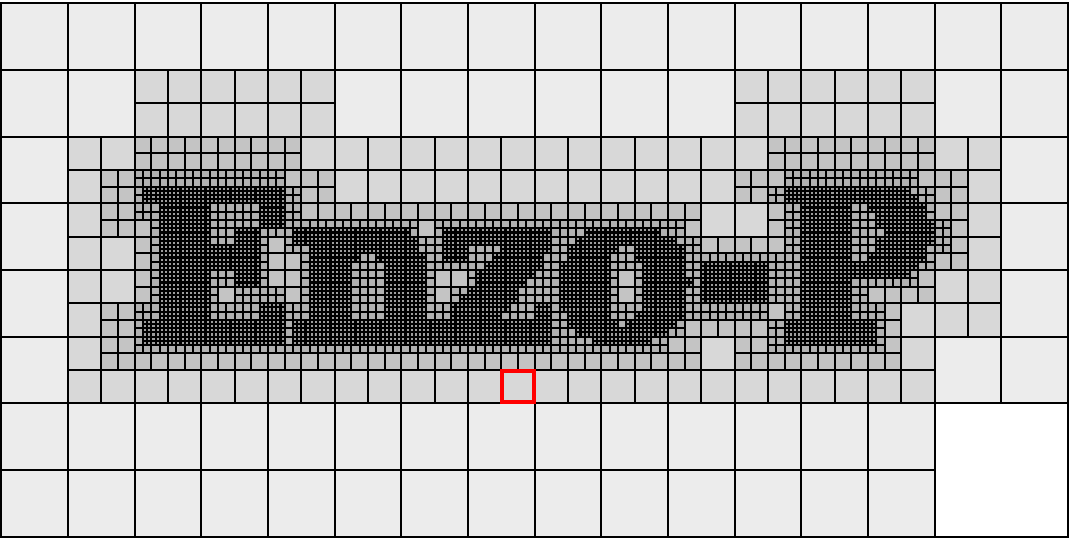
\includegraphics[width=2in]{amr-hierarchy.pdf}}
\end{minipage} \ \\ \vspace{0.1in}
\begin{minipage}{2.2in}
\centerline{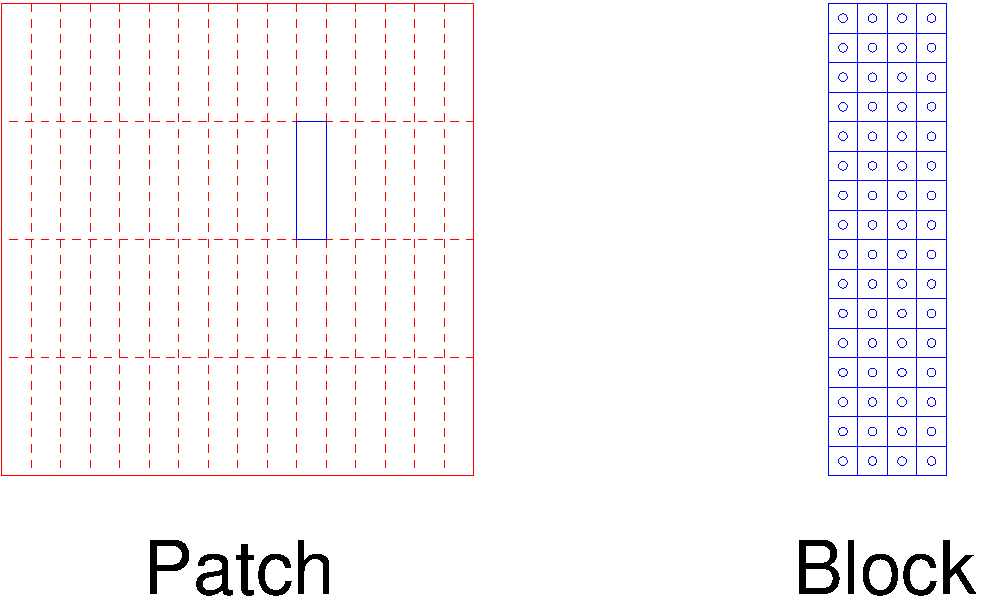
\includegraphics[width=1.6in]{amr-patch.pdf}}
\end{minipage} \ \\
\end{center}
\end{frame}

\begin{frame}[fragile] 
%--------------------------------------------------
\frametitle{\cello\ Mesh data structure}
\framesubtitle{\code{Mesh} related classes}
%--------------------------------------------------
%  AMR:        additional level of refinement: patches + blocks
%  AMR:        new [currently proprietary] enhancement for "large, shallow" AMR
%  AMR:        new [currently proprietary] enhancement for "deep, targeted" AMR
%  AMR:        no level jumps, symmetric refinement for symmetric problems
%  AMR:        ghost zones optionally allocated only when needed
\centerline{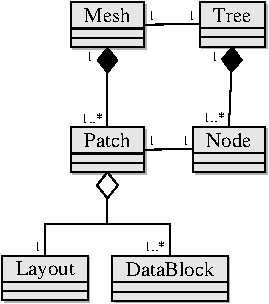
\includegraphics[width=2.5in]{uml/amr.pdf}}

\end{frame}

\begin{frame}[fragile] 
%--------------------------------------------------
\frametitle{\cello\ Mesh data structure}
\framesubtitle{\code{Mesh} related classes}
%--------------------------------------------------
%  AMR:        additional level of refinement: patches + blocks
%  AMR:        new [currently proprietary] enhancement for "large, shallow" AMR
%  AMR:        new [currently proprietary] enhancement for "deep, targeted" AMR
%  AMR:        no level jumps, symmetric refinement for symmetric problems
%  AMR:        ghost zones optionally allocated only when needed
\begin{itemize}
\small
\item \code{Mesh}: full AMR hierarchy
\item \code{Patch}: region of uniform resolution
  \begin{itemize}
  \item Cello unigrid problem degenerates to single \code{Patch}
  \end{itemize}
\item \code{Block}: basic distributed data unit / parallel task
  \begin{itemize}
  \item MPI: e.g.~one \code{Block} per process in Cartesian topology
  \item CHARM++: one \code{Block} per 3D ``chare array''
  \item GPU / OMP / UPC support planned
  \end{itemize}
\item \code{Layout}: specifies how to distribute \code{Block}s in a \code{Patch}
  \begin{itemize}
  \item \code{Block} size, process range, neighbor pointers, etc.
  \item hierarchical parallelism through multiple \code{Layout}s
  \end{itemize}
\item \code{Block} data: \code{Field}, \code{Particles}, etc.
\item \code{Tree}, \code{Node}: bare-bones octree data structure
  \begin{itemize}
  \item \code{Node}s are only objects replicated across machine
    \begin{itemize}
    \item small nodes: $\le 24$ bytes ($>1500$ bytes/\code{grid} for Enzo)
    \item fewer nodes: e.g.~$1$ instead of $P$ for unigrid case
    \end{itemize}
  \end{itemize}
\end{itemize}

\end{frame}






\section{Parallelization}
  \begin{frame}[fragile] 
%--------------------------------------------------
\frametitle{Dynamic scheduling}
%--------------------------------------------------
\begin{itemize}
\item\enzo\ grid patches proceed level-by-level
\begin{itemize}
\item   Static scheduling based on W-cycle through levels
\item   Bryan: ``refined patches work to catch up to their neighbors''
\item   Introduces artificial data dependencies
\end{itemize}
\begin{itemize}
\item      e.g. at first step, \textit{all} grids could advance
\item      slow localized region of domain can slow down entire simulation
\end{itemize}
\item\cello: patches advance dynamically
\begin{itemize}
\item   Bordner: ``patches work to get ahead of their neighbors''
\item   Dynamic scheduling based on data dependencies with neighbors
\begin{itemize}
\item     a patch can advance when all of its neighbors have caught up
\item     more forgiving for large processor counts
\end{itemize}
\end{itemize}
\end{itemize}
\end{frame}

\section{Conclusions}
  %------------------------------------------------------------------------
\begin{frame}[fragile] 
   \frametitle{Conclusions}


%   - Public website
%   - Developer website
%   - MPI-parallel unigrid Enzo PPM hydro "soon"
%   - Feedback desired
%     - parameters
%     - missing functionality?
%     - unnecessary functionality?
%     - easy of physics method development?


\begin{itemize}
\item Public \cello\ Trac site: \\ \textcolor{blue}{\url{http://lca.ucsd.edu/projects/cello}}
\item Current working draft of \enzop\ parameters:
{\footnotesize\colorcode{\url{http://lca.ucsd.edu/projects/cello/wiki/NotesParametersEnzo}}}
\end{itemize}
\begin{minipage}{2.6in}
\begin{itemize}
\item Feedback welcome--write me a ticket!
\begin{itemize}
\item parameter suggestions
\item missing features
\item ``that won't work!''
\item general observations
\end{itemize}
\end{itemize}
\end{minipage} \
\begin{minipage}{1.2in}
   \centerline{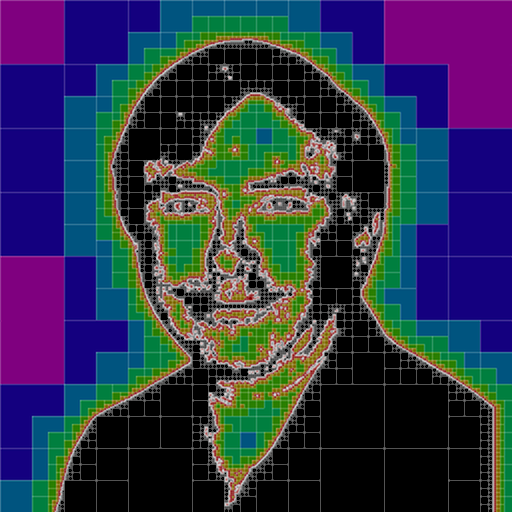
\includegraphics[width=1.2in]{norman.png}}
\end{minipage}
\ \\
\ \\
\centerline{$\qed$}
\end{frame}



\end{document}
